\newpage
\refstepcounter{section}
%Add Image
\vspace*{-40mm} %Make image have no top margin
\begin{tikzpicture}
\node[inner sep=0pt] (x) at (0,0)
    {\hspace{-87mm}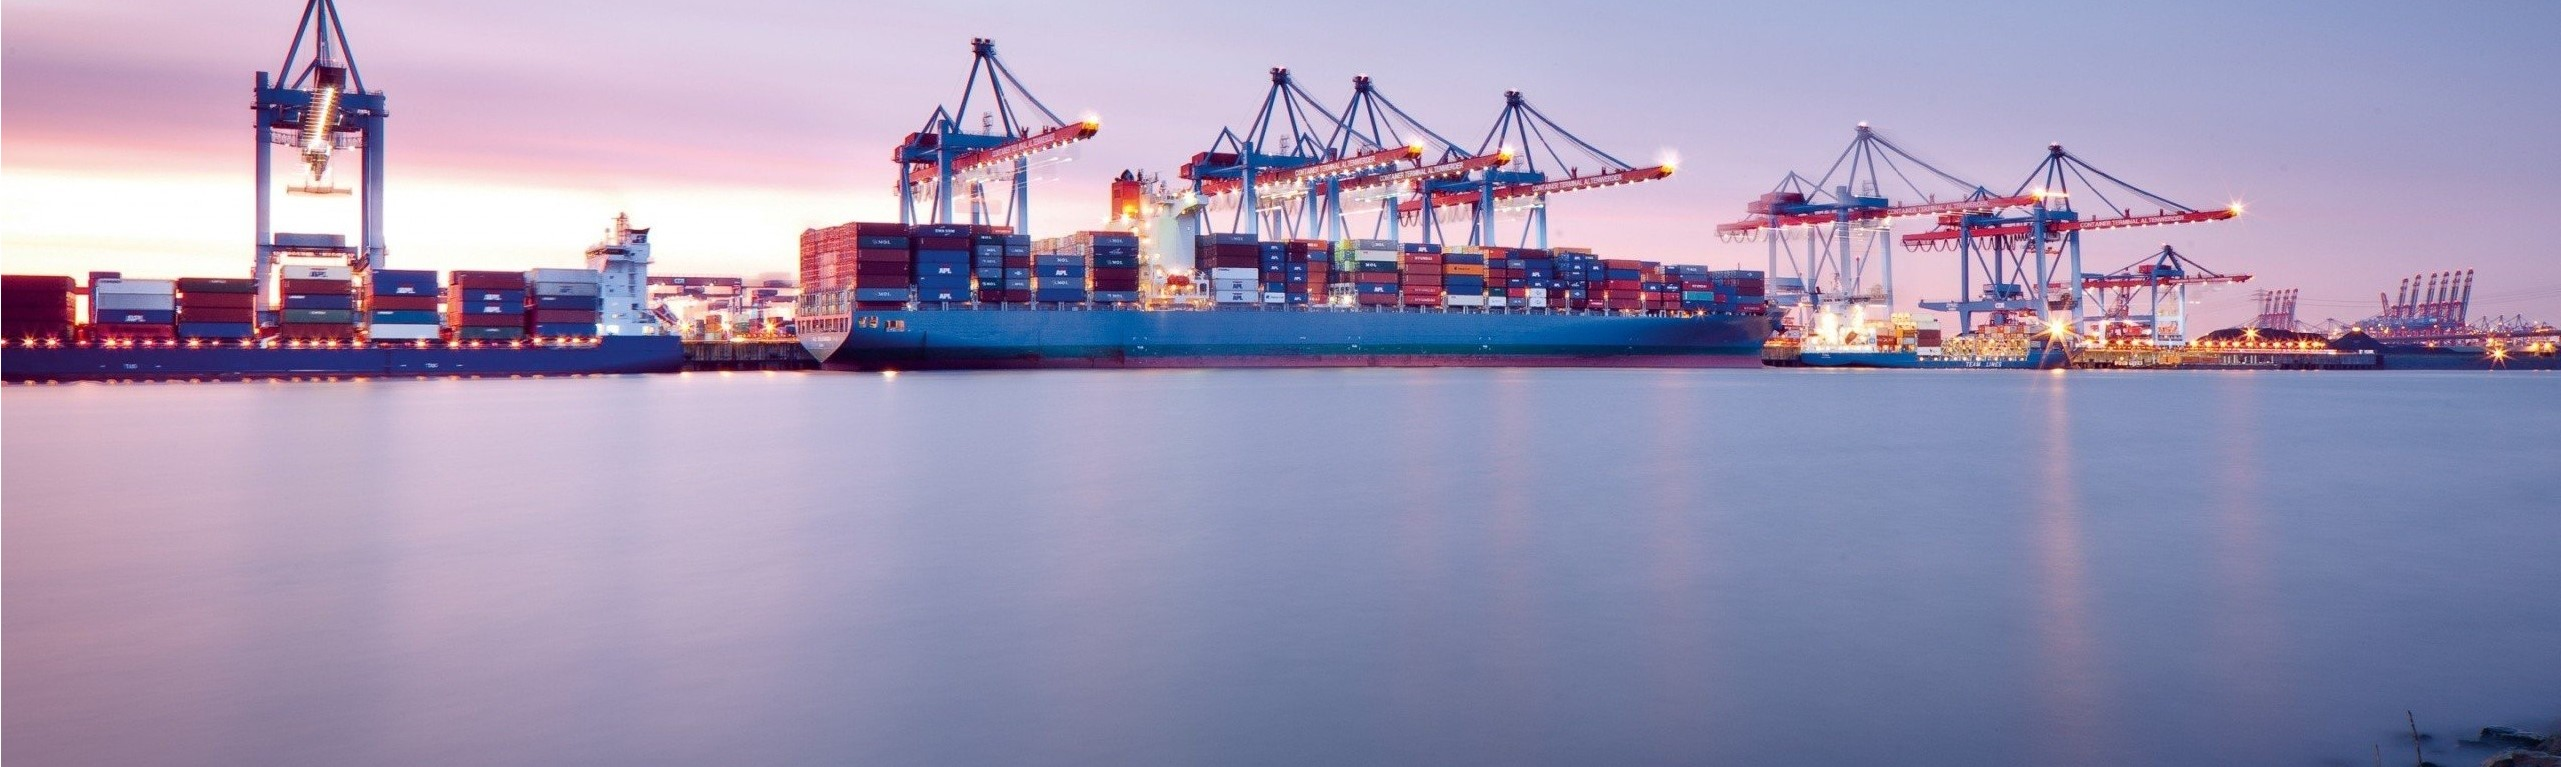
\includegraphics[width=\paperwidth]{sectionimage3.jpg}};
\node[text width=10in] (Z) at (0,-1) {\color{white}\headingfont\Large\bfseries\uppercase{\hspace{-0.7cm}\thesection\hspace{0.5cm}Implementation}};
\end{tikzpicture}
%Modify TOC
\addcontentsline{toc}{section}{\protect\numberline{\thesection}Implementation}
  \sectionmark{Implementation}




\subsection*{PHASE 1 - Planning of Project}
Planning of construction will begin in 2020 and last approximately five years. Phase I involves identifying the required equipment, workforce, materials, and other resources needed to complete the project. The project includes the expansion of Port of Tauranga (PoT), and rail and road development from Auckland to Tauranga via Hamilton.

\subsection*{PHASE 2 - Expansion of PoT and Construction of Road and Rail}
By 2025, planning will be complete, and construction will begin. The project will involve three sub-projects in total; the initial expansion of the PoT, lane additions on State Highway 29 (SH29), and the construction of a new railway track between Hamilton and Tauranga, including a new Kaimai Ranges tunnel. 
\\To facilitate the partial transition of freight from PoA to PoT, the capacity of the road and rail needs to be increased. State Highway 1 (SH1) to SH29 is the proposed route for trucks to transport freight between Tauranga and Auckland. SH1 is currently a four-lane-two-way highway while SH29 is only a two-lane-two way road. It is proposed to upgrade SH29 to a four-lane-two-way road over a three-year timeframe. The first expansion of the PoT occurs in conjunction with highway development. 
\\The decrease in freight at PoA will vacate prime real estate on the waterfront. Leasing real estate will generate revenue to fund the construction costs of both the SH29 and railway upgrade from Tauranga to Hamilton. Road upgrades have a smaller capital investment than the rail line construction, \$2.04 billion as opposed to \$5.62 billion. Refer to the CBA in the appendix for estimated costs.
During the upgrade of SH29 and the expansion of PoT, there will be an additional rail line constructed beside the East Coast Main Trunk Line, located between Claudelands and Tauranga. This additional line improves freight transport efficiency and introduces redundancy as a safety factor. A major cost to this additional rail line will be the second tunnel through the Kaimai Ranges. This will need to be done as the existing tunnel does not have the capacity to facilitate another rail line. 


\subsection*{PHASE 3 - Begin Incremental Freight Transition}
By 2028, the PoT initial expansion and the SH29 lane addition will be complete. The transition of freight from PoA to PoT will commence, with the 8\% annual freight transition beginning in 2028. This transition will continue for ten years, terminating in 2038, when 80\% of the original total freight of PoA, is transitioned to PoT. 
\\After the second year of transitioning freight, there will be 16\% less freight handled at PoA, which is assumed for this analysis to proportionally vacate 16\% of PoA rest estate on the waterfront, this will not be a realistic expectation. This real estate can then be leased for just over \$1 billion, a partial sum of this will be put back into the project. This leasing cycle can continue in two-year increments during the freight transition phase. 

Refer to CBA in Appendices for future cash flows up until the transition terminates and PoA is at 20\% capacity (year 2035).

\subsection*{PHASE 4 - Secondary PoT Expansion Commences}
The second expansion commences in 2035 and terminates in 2038 to cater for the remaining freight from PoA as rail is now fully developed. By 2038, 80\% of Auckland freight will have been transitioned to the PoT.

\subsection*{PHASE 5 - Performance Assessment}
With the completion of construction and expansions, past statistics and data on pollution, recurring costs, traffic congestion, and other factors will be used to estimate whether or not the project will remain successful in the future.
\\Delays or Disruptions:
To account for delays or disruptions, in our analysis of the NPV, we extended the project timeline to be completed in 2044.

\subsection*{Economic and Financial Analysis}
The implementation of the project will have a total cost of approximately \$15 billion. The initial cost for the first two years of this project is approximately \$4 billion. The revenue we receive from both the Port of Auckland and the Port of Tauranga, will be approximately \$1 billion. The remaining \$3 billion will be evenly distributed and invested by the Central Government and the Public-Private Partnership. This is an estimation, and is dependant on many factors. Investments will be made continuously throughout the ten years of construction with another \$350 million investment in 2035 to expand the port of Tauranga.
\\The largest area of expenditure for our project, is the operating costs from the rail and roading freight networks. Over the 25-year scope of our project, the calculated estimation of freight transport operating costs, is \$6.55 billion total. This accounts for 44\% of the total costs of the project. This is illustrated in the pie graph, and the other costs of the project are compared.

\subsection*{Cost Benefit Analysis}
    \subsubsection*{Financial Capital}
        \begin{itemize}[noitemsep]
            \item[] \textbf{Capital Cost}
            \item Road Expansion  -  \$2.04 Billion
            \item Rail Construction - \$5.6 Billion
            \item Port Expansion - \$700 million
            \item[] \textbf{Benefit}
            \item Port of Auckland \& Net Profit \$206 million PA with a growth rate of 8\%
            \item Benefit from Land of Port of Auckland \$7.3 billion
        \end{itemize}
    \subsubsection*{Natural Capital}
        \begin{itemize}[noitemsep]
            \item First 10 years of transition, an additional 139,500 tonnes of CO2 will be emitted by the increase of freight trucks. The estimated emission of CO2 is approximated to 51.2 million litres. Assuming the CO2 emitted correlates to the amount of fuel consumed the estimate environmental cost for this project is evaluated to \$82 million PA.
            \item After the completion of the electric railway system CO2 emission will be reduced by 21 million litres. This equates to approximately \$33.6 million PA for environmental benefit.
        \end{itemize}
        Natural Capital is the stock of natural resources. We quantified the release of carbon emissions as an environmental cost in our NPV calculations. These figures are estimated as accurate as possible with the data we have.
    \subsubsection*{Social/Human Capital}
        \begin{itemize}[noitemsep]
            \item Due to reduced traffic congestion each person saves 20 minutes per day. Assuming the average wage is \$23/hr, and half the population of Auckland (700,000) travels by road, the benefit from reduced traffic congestion evaluates to approximately \$1.4 billion PA.
            \item Total salary in PoT is currently \$32 million. Expansion of PoT will increase employment by 80\% measuring to approximately \$57.6 million PA. 
            \item The project will increase Tauranga's GDP by 2\%. The predicted contribution to GDP by this project, will be approximately \$1.4 billion, evaluating to \$28 million PA contributed by the increase of port operations.
        \end{itemize}
        Human capital and Social capital is the value added by the wider community and personal wellbeing. The reduction of traffic congestion improves the quality of life for daily commuters in Auckland. The expansion of the port will also significantly increase local employment and cash flow, promoting regional and urban development in Tarunga.
        
\begin{figure}
\centering
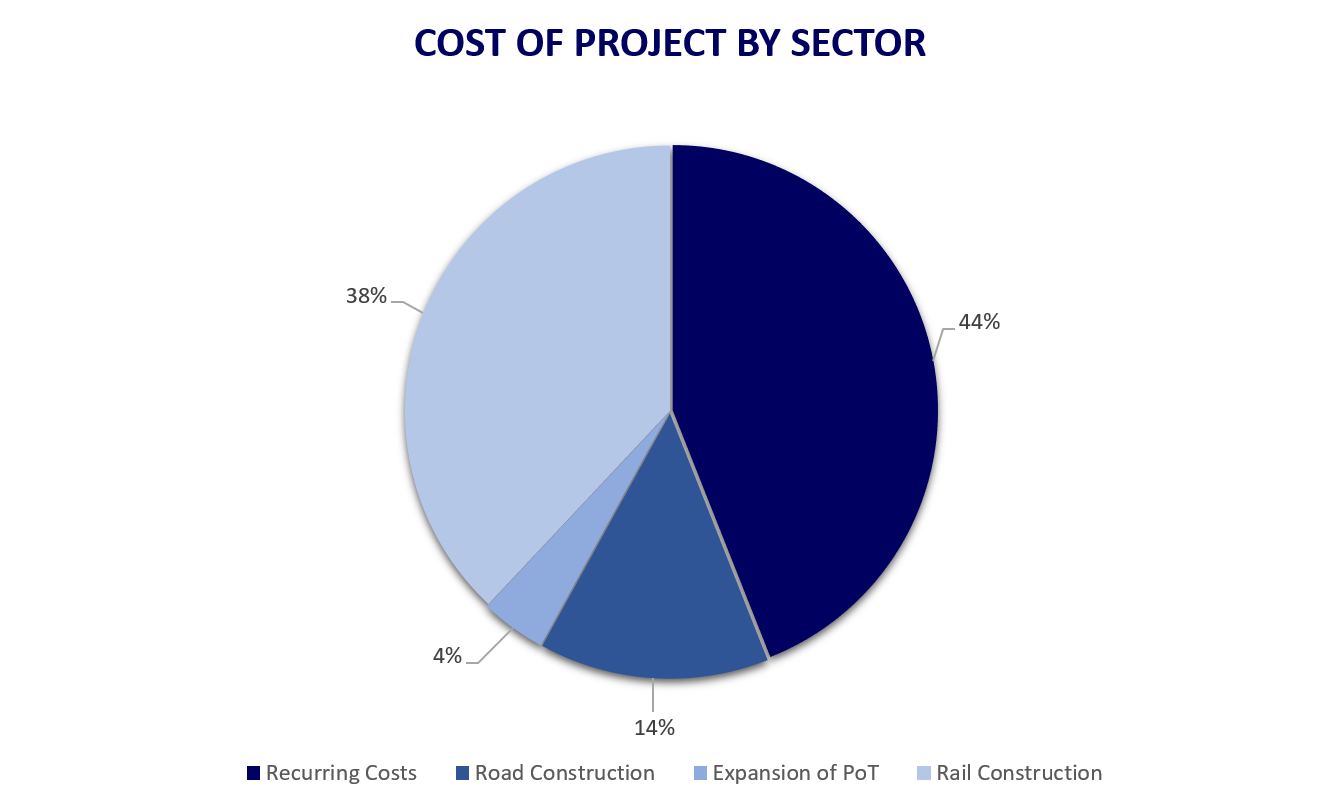
\includegraphics[width=0.9\textwidth]{CostBySector.png}
\centering
\caption{Cost of Project by Sector}
\end{figure}

% \newpage
\begin{figure}
\centering
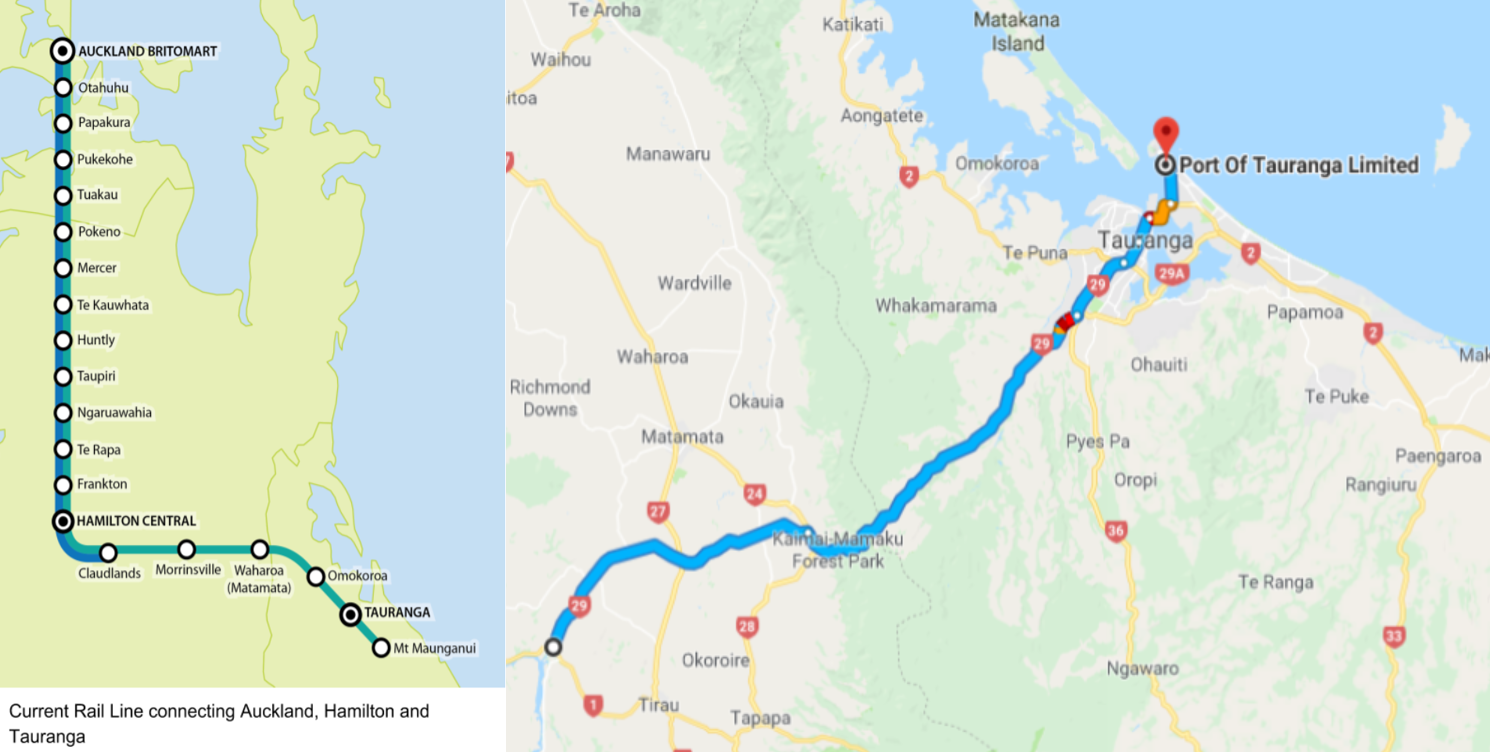
\includegraphics[width=0.9\textwidth]{implementationImage.png}
\centering
\caption{Current Rail Line/Road from Auckland to Tauranga}
\end{figure}

\begin{figure}
\centering
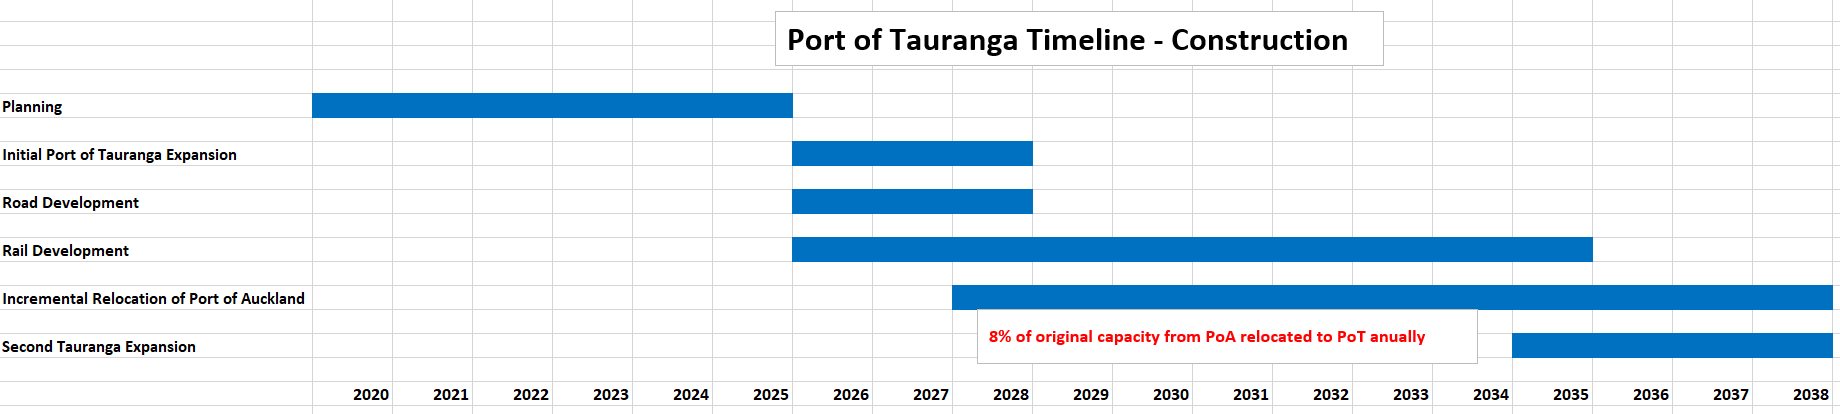
\includegraphics[width=0.9\textwidth]{Timeline.png}
\centering
\caption{Project Timeline}
\end{figure}

\clearpage